\documentclass[]{beamer}
% \geometry{papersize={16cm,9.60cm}}
\usepackage{etex}
\usepackage{amsmath}
\usepackage{tikz}
\usepackage{multimedia}
\usetheme{Boadilla}
\usepackage{graphicx}
\usepackage{url}
%\usepackage{inputenc}

% \mode<presentation>
% {
%   \usetheme{default}
%   \setbeamercovered{transparent}
% }


% {\vskip5pt}

%% customize layout, bullet points navigation toolbar
\setbeamertemplate{navigation symbols}{}%remove navigation symbols
\setbeamertemplate{enumerate items}[default]
\setbeamertemplate{navigation symbols}{}
\setbeamertemplate{itemize items}[circle]
\setbeamercolor{enumerate item}{fg=black}

\setbeamertemplate{footline}{}
\setbeamersize{text margin left = 2.0em}
\setbeamersize{text margin right = 2.0em}

\usepackage{times}
\usepackage[T1]{fontenc}

% Or whatever. Note that the encoding and the font should match. If T1
% does not look nice, try deleting the line with the fontenc.

\setbeamertemplate{navigation symbols}{}

\title{ Cognitive (Neuro) Psychology }
\subtitle{VII. Attention}
\author{ Marianne Maertens }
\institute[TU Berlin]{Technische Universit\"at Berlin}
\date{September 2016}

\begin{document}
\setbeamertemplate{enumerate items}[default]
\setbeamertemplate{headline}

\frame{\titlepage}

\AtBeginSection[]
{
  \begin{frame}<beamer>
    \frametitle{Layout}
    \tableofcontents[currentsection]
  \end{frame}
}


\begin{frame}
 \frametitle{Objectives}
\begin{overlayarea}{110mm}{70mm}
 basic knowledge in
\begin{itemize}
  \item Cognitive (Neuro) \textbf{Psychology}
  \item Experimental Methods
\end{itemize}

\vspace{5mm}
\only<2->{
\begin{itemize}
 \item[$\Rightarrow$] What kind of questions are addressed in the discipline?
 \item[$\Rightarrow$] How are these questions being addressed?
 \item[$\Rightarrow$] Be able to comprehend and evaluate literature and work done in the field.
\end{itemize}
}
\end{overlayarea}
\end{frame}

\begin{frame}
 \frametitle{Topics \& Structure}
\includegraphics<1>[width=120mm]{figs/l7/timetable.pdf} 
\end{frame}


\begin{frame}
 \frametitle{Philosophy}
\begin{overlayarea}{110mm}{50mm}
Challenge: block course!! \\
\vspace{5mm}
\only<2->{
 \begin{itemize}
  \item alternation between instruction and individual studies
  \item active involvement of participants
  \item some topics in depth instead of broad coverage
  \item exam: indicate the degree of retention of material - MC 
  \item[]
  \item<3->[?] Comments, Questions?
 \end{itemize}
}
\end{overlayarea}
\end{frame}


\begin{frame}
\begin{center}
 \begin{LARGE}
What happened so far? 
\end{LARGE}
 \end{center}
\end{frame}


\begin{frame}{Recap}
 \begin{overlayarea}{110mm}{70mm}
  \begin{columns}[T]
   \begin{column}{60mm}
    \begin{itemize}
     \item Experimental methodology
    \begin{itemize}
     \item<1-> Hypothesis, experimental design, etc.
     \item<2-> Psychophysics, thresholds, sensitivity
     \item<3-> Measuring appearance 
    \end{itemize}
   \item<4-> Visual information processing
    \begin{itemize}
     \item<4-> Properties of visual neurons, orientation selectivity, spatial frequency selectivity, ...
     \item<5-> Visual functions, orientation discrimination, acuity, ...
     \item<6-> Object recognition
    \end{itemize}
   \end{itemize}
   \end{column}

   \begin{column}{50mm}
    \begin{center}
    \includegraphics<1>[width=50mm]{../../../figures/huber_hypothesis.png}
   \includegraphics<2>[width=40mm]{../../../figures/muller_lyer_pmf_pse.png}
   \includegraphics<3>[width=40mm]{figs/l6/knoblauch_scaling98.png}
   \includegraphics<4>[width=40mm]{figs/l5/ventral_pathways.png}
   \includegraphics<5>[width=40mm]{figs/l3/csf_demo.png}
   \includegraphics<6>[width=50mm]{figs/l5/T_junctions.png}
   \end{center}
  \end{column}
  \end{columns}
 \end{overlayarea}
\end{frame}


\begin{frame}
 \begin{center}
\includegraphics<1>[width=50mm]{figs/l8/serial_reading.png}
\includegraphics<2->[width=115mm]{figs/l8/waldo.png}
 \end{center} 
\end{frame}


\begin{frame}
 \frametitle{Attention}
\begin{overlayarea}{110mm}{80mm}
 \begin{itemize}
  \item a very large set of selective processes in the brain
 \item[] 
 \item<2-> impossible to handle all inputs at once
 \item<2-> nervous system has evolved mechanisms that are able to restrict processing to a subset of things, places, ideas, moments in time
 \end{itemize}
\only<3->{
\textcolor{blue}{Selective Attention}
 \begin{itemize}
  \item form of attention involved when processing is restricted to a subset of possible stimuli
\end{itemize}
}
 \begin{center}
 \end{center} 
\end{overlayarea}
 \end{frame}

\begin{frame}
\frametitle{Selective Attention}
 \begin{center}
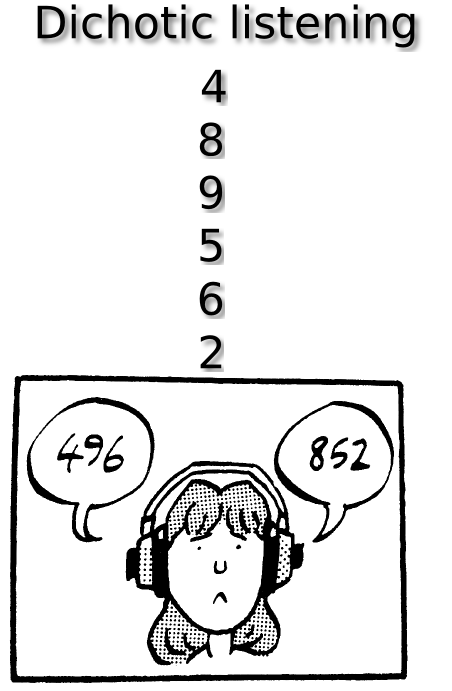
\includegraphics[width=35mm]{figs/l1/dichotic_listening_task.png}
 \end{center} 
\end{frame}


\begin{frame}
 \frametitle{Overview}
\begin{itemize}[<+->]
  \setlength{\itemsep}{5pt}
 \item Experimental paradigms for studying attention
 \begin{itemize}
  \item in space
  \item in time
 \end{itemize}
 \item Physiological basis of attention
 \item Disorders of attention
 \item Scene perception
\end{itemize}
\end{frame}

\begin{frame}
\frametitle{Attention}
\begin{overlayarea}{110mm}{80mm}
\begin{itemize}
 \item<1-> not a single \textit{thing} and does not have a single locus in the brain: pay attention, be alert, concentrate ...
 \item[]
 \item<2-> external vs. internal
 \item<3-> overt vs. covert (with vs. without eye movements)
 \item<4-> focussed vs. divided
 \item<5-> sustained
 \item<6-> selective
\end{itemize}
\end{overlayarea}
\end{frame}


\begin{frame}
 \frametitle{Selection in space}
\begin{overlayarea}{130mm}{75mm}
\only<1->{
\begin{itemize}
 \item[] What does it mean to ``pay attention``?
\end{itemize}
}
\only<2->{
\begin{center}
\textcolor{blue}{Cueing paradigm} \begin{scriptsize}(Posner, 1980) \end{scriptsize}

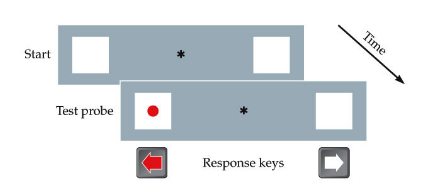
\includegraphics[width=80mm]{figs/l8/cueing_basic.png}
\end{center}
}

\only<3->{
Hit a response key as fast as possible when the probe appears!\\
\textbf{Dependent variable:} reaction time (RT)
}
\end{overlayarea}
\end{frame}



\begin{frame}
 \frametitle{Selection in space}
\begin{overlayarea}{110mm}{75mm}

\begin{center}
\textcolor{blue}{Cueing paradigm} \begin{scriptsize}(Posner, 1980) \end{scriptsize}
\end{center}
\begin{columns}[T]
 \begin{column}{50mm}
\centering valid
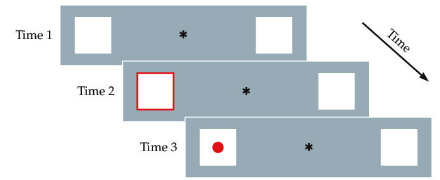
\includegraphics[width=60mm]{figs/l8/cueing_valid.png}
 \end{column}

 \begin{column}{80mm}
\centering invalid
 
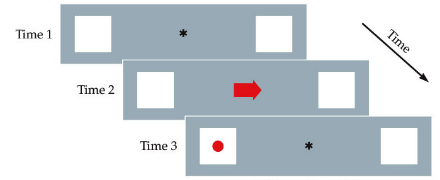
\includegraphics[width=60mm]{figs/l8/cueing_invalid.png}
 \end{column}
\end{columns}

\vspace{5mm}
\begin{itemize}
 \item<2->[Cue] stimulus that indicates where (or what) subsequent stimulus might be. Valid (giving correct information), invalid or neutral.
 \item<3-> exogeneous/peripheral vs. endogeneous/symbolic cues
 \item<4->[SOA] stimulus onset asynchrony  - time between onset of one stimulus and onset of another.
\end{itemize}
\end{overlayarea}
\end{frame}


\begin{frame}
\frametitle{Selection in scace}
\begin{overlayarea}{110mm}{80mm}
\begin{center}
\textcolor{blue}{Cueing paradigm} \begin{scriptsize}(Posner, 1980) \end{scriptsize}
\end{center}

 \begin{center}
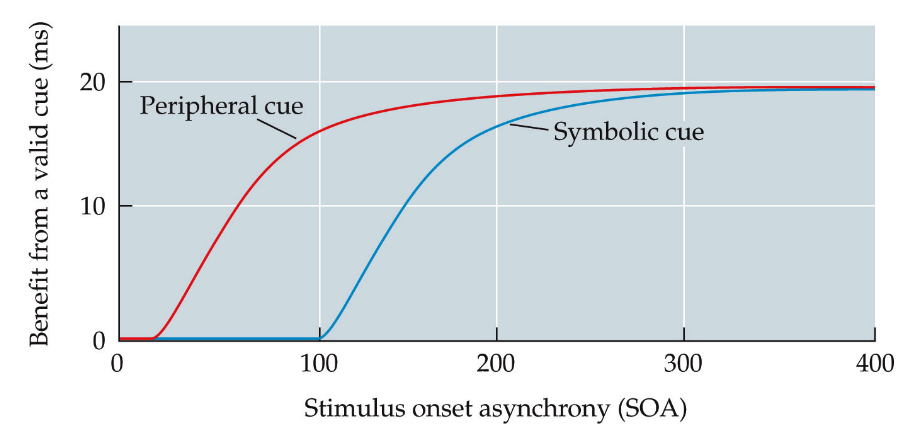
\includegraphics[width=70mm]{figs/l8/cueing_results.png}
 \end{center}

\begin{columns}[T]
 \begin{column}{80mm}
 \begin{itemize}
 \item benefit from valid cue: $RT_{invalid} - RT_{valid}$
 \item increases with processing time for cue 
 \item peripheral cue is processed quicker
\end{itemize}
 \end{column}

 \begin{column}{40mm}
\includegraphics<2->[width=30mm]{figs/l8/symbolic_cue.png}  
 \end{column}
\end{columns}
\end{overlayarea}
\end{frame}



\begin{frame}
\frametitle{Metaphors of Attention}
\begin{overlayarea}{110mm}{75mm}
\textbf{Spotlight model:}

\begin{itemize}
 \setlength{\itemsep}{5pt}
 \item attention is restricted in space and moves from one point to the next
 \item in-depth processing of areas within spotlight
\end{itemize}

\textbf{Zoom lens model:}

\begin{itemize}
 \setlength{\itemsep}{5pt}
 \item attended region can grow or shrink depending on the size of the area to be processed in detail
\end{itemize}
\end{overlayarea}
\end{frame}


\begin{frame}
 \frametitle{Visual Search}
\begin{overlayarea}{120mm}{70mm}
closer approximation of deployment of attention in the real world
\vspace{4mm}
\begin{columns}[T]
 \begin{column}{50mm}
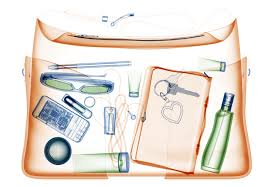
\includegraphics[width=40mm]{figs/l8/suitcase_scan.jpg}
 \end{column}

 \begin{column}{60mm} 
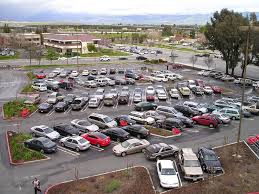
\includegraphics[width=40mm]{figs/l8/car_in_parking_lot.jpg}
 \end{column}
\end{columns}

\vspace{4mm}
Find the \textit{target} item among \textit{distractor} items!
\begin{itemize}
 \item[] 
 \item<2->[] \textbf{target} - goal of visual search
 \item<2->[] \textbf{distractor} - any stimulus other than the target (in visual search)
 \item<2->[] \textbf{set size} - number of items in visual search display
\end{itemize}
\end{overlayarea}
\end{frame}

\begin{frame}
 \frametitle{Visual search}
\includegraphics<1>[width=110mm]{figs/l8/types_visual_search_displays.png}
\includegraphics<2>[width=110mm]{figs/l8/types_visual_search.png}
\end{frame}

\begin{frame}
 \frametitle{Visual Search}
\begin{center}
\includegraphics<1>[width=100mm]{figs/l8/types_visual_search_summary.png}
\end{center}

Efficiency is quantified as average RT as a function of set size 
\begin{itemize}
  \item search slope, $\frac{ms}{item}$
  \item the larger the slope the less efficient the search
 \end{itemize}
\end{frame}



\begin{frame}
\begin{block}{Activity}
Quantify your visual search performance in the activity on the following webpage \url{http://sites.sinauer.com/wolfe4e/wa07.02.html}.\\ Do 15 trials in each condition.
 \end{block}
\end{frame}


\begin{frame}
 \frametitle{Using search efficiency to explore visual processing}
\begin{overlayarea}{110mm}{70mm}
\begin{columns}[T]
\begin{column}{40mm}
\includegraphics<1>[width=40mm]{figs/l8/feature_search.png}
\includegraphics<2>[width=40mm]{figs/l8/enns_rensink.png}
\end{column}

\begin{column}{70mm}
\begin{itemize}
 \item \textbf{feature search} - target defined by presence of single feature
 \item ''pop out`` of the target because of its saliency
 \item color or orientation can be processed at once - \textbf{parallel} search 
 \item[]
 \item<2-> look for the odd one out
 \item<2-> overall shape and orientation same, 
 \item<2-> difference in perceived depth \textbf{feature difference}
\end{itemize}
\end{column}
 \end{columns}
\end{overlayarea}
\end{frame}


\begin{frame}
 \frametitle{Using search efficiency to explore visual processing}
\begin{overlayarea}{110mm}{70mm}
\begin{columns}[T]
\begin{column}{40mm}
\includegraphics<1>[width=40mm]{figs/l8/serial_search.png}
\includegraphics<2>[width=40mm]{figs/l8/chinese_search.png}
\end{column}

\begin{column}{70mm}
\begin{itemize}
 \item \textbf{conjunction search} - target defined by co-occurrence of more than one feature
 \item each additional distractor adds a fixed amount of search time
 \item slope in trials without target twice as large as slope in trials with target 
 \item target absent:present 50:50
 \item[$\rightarrow$] \textbf{serial self-terminating} search
 \item[]
 \item<2-> hardest search except you read Chinese
 \item<2-> T-among-L is simpler ''target hides in plain sight''
\end{itemize}
\end{column}
 \end{columns}
\end{overlayarea}
\end{frame}

\begin{frame}
 \frametitle{Real-world searches}
\begin{center}
\includegraphics<1>[width=80mm]{figs/l8/real_world_search.png}
\end{center}
In real-life search is often \textbf{guided:} Attention is restricted to a subset of possible items on the basis of information about the target's basic features (e.g., its color)
\end{frame}

\begin{frame}
 \frametitle{Attending in time}
\textbf{Rapid Serial Visual Presentation (RSVP)} - experimental procedure in which stimuli appear in a stream at one location at a rapid rate
\begin{itemize}
 \item decide whether there was an X in the stream of letters
 \item 8-10 items per second, every 120-125ms 
\end{itemize}
\end{frame}



\begin{frame}
 \frametitle{Rapid Serial Visual Presentation (RSVP)}
\begin{overlayarea}{120mm}{80mm}
\begin{center}
\includegraphics<1>[width=80mm]{figs/l8/rsvp.png}
\end{center}

\only<2->{
\textbf{Attentional blink} - tendency not to perceive a target when it is presented 200-500ms after another target within a rapid stream of distractors
\begin{columns}[T]
\begin{column}{50mm}
\includegraphics<2->[width=60mm]{figs/l8/attentional_blink.png}
\end{column}

\begin{column}{60mm}
 \begin{itemize}
  \item T2 is missed when T1 is correctly reported
  \item T2 is detected when it appears immediately after T1
  \item reduced attentional blink for experienced video game players
 \end{itemize}
\end{column}
\end{columns}
}
\end{overlayarea}
\end{frame}



\begin{frame}
\begin{block}{Activity}
Explore RSVP and attentional blink in the follwing web activities  \url{http://sites.sinauer.com/wolfe4e/wa07.03.html} and \url{http://sites.sinauer.com/wolfe4e/wa07.04.html}
 \end{block}
\end{frame}


\begin{frame}
 \frametitle{Neurophysiological basis of attention}
\begin{overlayarea}{120mm}{80mm}
 "Everyone knows what attention is. ... It is the taking possession by the mind, in clear and vivid form, of one out of several possible trains of thought`` (James, 1890)\\
\vspace{3mm}

\only<2->{What is the brain doing when it selects one location in space, one object, or one moment in time?}

\begin{columns}[T]
 \begin{column}{35mm}
\includegraphics<3>[width=35mm]{figs/l8/fmri_spatial_attention.png}
\begin{center}
\includegraphics<4->[width=55mm]{figs/l8/fmri_object_attention.png}
\end{center}
 \end{column}

 \begin{column}{75mm}
\begin{itemize}
 \setlength{\itemsep}{8pt}
 \item<3-> attending to different locations as in Posner cueing task -  corresponding activity in retinotopic areas
 \item<4-> attending to different categories - activity in different brain areas:
\begin{itemize} 
 \item[] Fusiform Face Area (FFA) 
 \item[] Parahippocampal Place Area (PPA)
\end{itemize}
\end{itemize}
 \end{column}
\end{columns}
\end{overlayarea}
\end{frame}

\begin{frame}
 \frametitle{Neurophysiological basis of attention}
\begin{overlayarea}{120mm}{60mm}

What is the brain doing when it selects one location in space, one object, or one moment in time?

\begin{center}
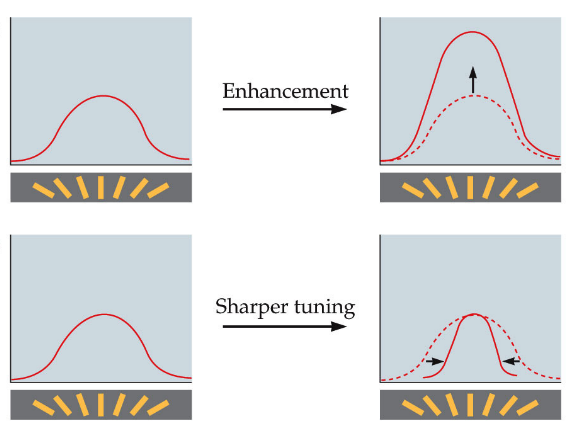
\includegraphics[width=60mm]{figs/l8/attention_tuning.png}
\end{center}
\end{overlayarea}
\end{frame}


\begin{frame}
 \frametitle{Disorders of Visual Attention}
\begin{overlayarea}{120mm}{75mm}
What would happen if you could longer pay attention? \\
\vspace{3mm}
\textbf{Visual field defect} - portion of the visual field with no vision due to damage to part of the visual nervous system\\
\vspace{3mm}
\only<2->{
\textbf{Visual (hemi)neglect} - inability of attend or respond to stimuli in the contralesional visual field (typical left) after lesions to the right parietal lobe}

\only<5->{
\vspace{3mm}
\textbf{Extinction} - inability to perceive a stimulus to one side of the midline in the presence of another stimulus}

\begin{columns}[T]
 \begin{column}{40mm}
\begin{center}
\includegraphics<3-4>[width=40mm]{figs/l8/neglect_right_IPL.jpg}
\end{center}
 \end{column}

 \begin{column}{70mm}
\begin{center}
\includegraphics<3>[width=60mm]{figs/l8/line_cancellation.png}
\includegraphics<4>[width=60mm]{figs/l8/copying.png}
\end{center}
 \end{column}
\end{columns}
\end{overlayarea}
\end{frame}

\begin{frame}
 \frametitle{The role of attention in scene perception}
\begin{overlayarea}{120mm}{60mm}

\textbf{Change blindness} (Rensink, O'Reagan and Clarke, 1997)
\begin{center}
\includegraphics<1>[width=60mm]{figs/l8/globe_and_high_court1.jpg}
\includegraphics<2>[width=60mm]{figs/l8/change_between.png}
\includegraphics<3>[width=60mm]{figs/l8/globe_and_high_court2.jpg}
\end{center}
\end{overlayarea}
\end{frame}


\begin{frame}
 \frametitle{The role of attention in scene perception}
\begin{overlayarea}{120mm}{60mm}
\textbf{Inattentional blindness} (Simon and Chabris, 1999)

\begin{center}
\includegraphics<1>[width=60mm]{figs/l8/inattentional_blindness.jpg}
\end{center}
\end{overlayarea}
\end{frame}


\begin{frame}
 \frametitle{Summary}
\begin{itemize}
\setlength{\itemsep}{5pt}
 \item \textit{attention} refers to large set of selective mechanisms that enable us to focus on some stimuli at the expense of others
 \item efficient and inefficient visual search performance informs us about ease of processing of object features
 \item attention varies over time and space, there is an attentional bottleneck between 200-500ms after stimulus processing
 \item effects of attention manifest themselves in different ways in the brain
 \item damage to the parietal lobe of the brain produces deficits in visual attention
 \item scene processing depends on attention - not see the forest for the trees ...
\end{itemize}
\end{frame}


\begin{frame}
 \frametitle{References}
\begin{small}
\begin{itemize}
 \item  Wolfe, J.M., Kluender, K.R. \& Levi, D.M. (2012).\textit{Sensation \& Perception}. Sinauer Associates: Sunderland, MA. 
\end{itemize}
\end{small}
\end{frame}


\end{document}